\documentclass[12pt]{article}
\usepackage{amsmath}
\usepackage{enumitem}
\usepackage{fixmath}
\usepackage{amsfonts}
\usepackage{graphicx}
\usepackage{xcolor}
\definecolor{colorsrc}{rgb}{0.36, 0.54, 0.66}

% \definecolor{colornan}{rgb}{0.5, 0.5, 0.5}
% \definecolor{colornan}{rgb}{0.43, 0.21, 0.1}
% \definecolor{auburn}{rgb}{0.43, 0.21, 0.1}
% \definecolor{colorwnd2}{rgb}{1, .44, .37}
\definecolor{colorlcksvd}{rgb}{0.91, 0.84, 0.42}
\definecolor{colorlcksvdd}{rgb}{0.8, 0.0, 0.1}
\definecolor{colorlcksvd}{rgb}{1, 0.56, 0.0}
% \definecolor{colornan}{rgb}{0, 0.8, 0.0}
% \definecolor{colorsrc}{rgb}{0.5, 1, 0}
% \definecolor{colorfdd}{rgb}{0.6, 0.4, 0.8}
% \definecolor{colorfdd}{rgb}{0.93, 0.53, 0.18}
\definecolor{colorfddl}{rgb}{0.44, 0.16, 0.39}
\definecolor{colordlsi}{rgb}{0.55, 0.71, 0.0}
% \definecolor{colorlck}{rgb}{0.43, 0.21, 0.1}
% \definecolor{colorlck}{rgb}{0.89, 0.82, 0.04}
% \definecolor{colorlck}{rgb}{0.03, 0.27, 0.49}
\definecolor{colorcopar}{rgb}{0.9, .0, 0}
% \definecolor{colorlrsd}{rgb}{0.72, 0.53, 0.04}
\definecolor{colorjdl}{rgb}{0.0, 0.55, 0.55}
\definecolor{colordlr}{rgb}{0.0, 0.55, 0.55}
\definecolor{colorlrsdl}{rgb}{0.0, 0.2, 1.0} % blue
% \definecolor{colorlck}{rgb}{0.5, 0.5, 0.0}
% \definecolor{colorlck}{rgb}{0.0, 0.42, 0.24}
\definecolor{colorlck}{rgb}{0.0, 0.9, 0.9}
\definecolor{pinegreen}{rgb}{0.0, 0.47, 0.44}

\def\myaddplotlrsdl{\addplot+[thick, colorlrsdl, solid, mark = square*, mark size=1.4, mark options={colorlrsdl}]}
\def\myaddplotfddl{\addplot+[thick, colorfddl, mark = diamond*, mark size=1.4, mark options={colorfddl}]}
\def\myaddplotlcksvd{\addplot+[thick, colorlcksvd, mark = x, mark size=1.8, mark options={colorlcksvd}]}
\def\myaddplotlcksvdd{\addplot+[thick, green, mark = triangle, mark size=1.4, mark options={green}]}
\def\myaddplotdlsi{\addplot+[thick, colordlsi, mark = *, mark size=1.4, mark options={fill = white}]}
\def\myaddplotsrc{\addplot+[thick, colorsrc, mark = square, mark size=1.4, mark options={colorsrc}]}
\def\myaddplotcopar{\addplot+[thick, colorcopar, solid, mark = *, mark size=1.4, mark options={colorcopar}]}
\def\myaddplotjdl{\addplot+[thick, pinegreen, solid, mark = diamond*, mark size=1.4, mark options={pinegreen}]}
\def\myaddplotdlr{\addplot+[thick, cyan, solid, dashed, mark = triangle*, mark size=1.4, mark options={cyan}]}


% \def\myaddplotcopar{\addplot+[colorcopar, mark = square*, mark options={colorcopar}]}
% \def\myaddplotdfd{\addplot+[colordfd,  mark options={colordfd}]}
% \def\myaddplotfdd{\addplot+[colorfdd,  mark options={colorfdd}]}
% \def\myaddplotlck{\addplot+[colorlck,  mark options={colorlck}]}
% \def\myaddplotnan{\addplot+[colornan,  mark options={colornan}]}
% \def\myaddplotwnd{\addplot+[colorwnd,  mark options={colorwnd}]}
% \def\wnd{{black,fill=colorwnd}}

\def\x{{\mathbf x}}
\def\L{{\cal L}}

\newcommand{\vect}[1]{\mathbf{#1}}

\newcommand{\mat}[1]{\mathbf{#1}}
\newcommand{\abs}[1]{\left|#1\right|}
\newcommand{\norm}[1]{\left\|#1\right\|}
% \newcommand{\R}{\mathbb{R}}
\newcommand{\Z}{\mathbb{Z}}
\newcommand{\tb}{\textbf}


\def\bmt{\left[\begin{matrix}}
\def\dpcm{$\square$}
\def\emt{\end{matrix}\right]}
% \def\proof{\underline{Proof:}\\}
\def\dpcm{$\square$}
\def\half{\frac{1}{2}}
\def\imply{\Rightarrow}
\def\foralli{\forall i = 1, 2, \dots, n}
\def\im{\mathrm{im}}
\def\ker{\mathrm{ker}}
\def\eqv{\Leftrightarrow}
\def\tcg{\textcolor{newgreen}}
\def\mb{\mathbf}
\def\tb{\textbf}
\def\mb {\mathbf}
\def\mc {\mathcal}
\def\tcb{\textcolor{blue}}
\def\tcg{\textcolor{green}}
\def\tcr{\textcolor{red}}
\def\tcgr{\textcolor{gray}}
\def\bx{\mathbf{x}}
% \def\bW{\mathbf{W}}
\def\ba{\mathbf{a}}
\def\bb{\mathbf{b}}
\def\bc{\mathbf{c}}
\def\bd{\mathbf{d}}
\def\be{\mathbf{e}}
\def\fb{\mathbf{f}}
\def\bg{\mathbf{g}}
\def\bh{\mathbf{h}}
\def\bm{\mathbf{m}}
\def\M{\mathcal{M}}
\def\bp{\mathbf{p}}
\def\bq{\mathbf{q}}
\def\bs{\mathbf{x}}
\def\bu{\mathbf{u}}
\def\bv{\mathbf{v}}
\def\by{\mathbf{y}}
\def\bz{\mathbf{z}}
\def\and{\text{~and~}}
\def\barN{\bar{N}}
\def\barNi{\bar{N}_i}
\def\trace{\textrm{trace}}
\def\etal{\textit{et al.}}
\def\R{\mathbb{R}}

\def\bzeros{\mathbf{0}}

\def\bA{\mathbf{A}}
\def\bB{\mathbf{B}}
\def\bD{\mathbf{D}}
\def\bE{\mathbf{E}}
\def\Fb{\mathbf{F}}
\def\bG{\mathbf{G}}
\def\bL{\mathbf{L}}
\def\bH{\mathbf{H}}
\def\bI{\mathbf{I}}
\def\bJ{\mathbf{J}}
\def\bM{\mathbf{M}}
\def\bN{\mathbf{N}}
\def\bP{\mathbf{P}}
\def\bQ{\mathbf{Q}}
\def\bR{\mathbf{R}}
\def\bS{\mathbf{S}}
\def\bU{\mathbf{U}}
\def\bV{\mathbf{V}}
\def\bW{\mathbf{W}}
\def\bX{\mathbf{X}}

\def\bY{\mathbf{Y}}
\def\bZ{\mathbf{Z}}
\def\rank{\text{rank}}
\def\bDi{\mathbf{D}_i}
% \def\bSi{\mathbf{X}_i}
\def\bXi{\mathbf{X}_i}
% \def\bSi{\mathbf{X}_i}
\def\barX{\bar{\mathbf{X}}}
\def\barD{\bar{\mathbf{D}}}
\def\barX{\bar{\mathbf{X}}}
\def\barXi{\bar{\mathbf{X}}_i}
\def\barDi{\bar{\mathbf{D}}_i}
\def\barXi{\bar{\mathbf{X}}_i}
\def\bW{\mathbf{W}}
\def\bw{\mathbf{w}}

\def\la{\langle}
\def\ra{\rangle}

\def\bDc{\bD_{0}}
\def\bXc{\bX^{0}}
\def\mM{\mathcal{M}}
\def\wt{\widetilde}

\def\bbX{\lbar{\bX}}        
\def\bbx{\lbar{\bx}}        
\def\bbY{\lbar{\bY}}        
\def\bbD{\lbar{\bD}}  

%% ================== block: Slide footnotes ==========================
\def\footnoteSRC{\setcounter{footnote}{3}\footnote[frame]{\tiny J. Wright et al., Robust face recognition via sparse representation, IEEE TPAMI, 2009}}
\def\footnoteLLC{\setcounter{footnote}{4}\footnote[frame]{\tiny  H. Zhang et. al., Locality-constrained linear coding for image classification, CPVR 2010}}
\def\footnoteJSRC{\setcounter{footnote}{5}\footnote[frame]{\tiny  Yen, Multi-View Automatic Target Recognition using Joint Sparse Representation, Aerospace and Electronic Sys. 2012}}
\def\footnoteJDSRC{\setcounter{footnote}{6}\footnote[frame]{\tiny  J. Wang et. al., Joint dynamic sparse representation for multi-view face recognition,  PR 2012}}
\def\footnoteSHIRC{\setcounter{footnote}{7}\footnote[frame]{\tiny U. Srinivas et. al., Simultaneous sparsity model for histopathological image representation and classification, TMI 2014}}
\def\footnoteKSVD{\setcounter{footnote}{8}\footnote[frame]{\tiny  M. Elad et. al., K -SVD: An Algorithm for Designing Overcomplete Dictionaries for Sparse Representation, TSP 2006 }}
\def\footnoteODL{\setcounter{footnote}{9}\footnote[frame]{\tiny J. Mairal et. al., Online learning for matrix factorization and sparse coding, JMLR 2010}}
\def\footnoteDKSVD{\setcounter{footnote}{10}\footnote[frame]{\tiny  Q. Zhang, B. Li, Discriminative K-SVD for dictionary learning in face recognition, CVPR 2010 }}

\def\footnoteLCKSVD{\setcounter{footnote}{11}\footnote[frame]{\tiny  Z. Jiang et. al., Label consistent K-SVD: Learning a discriminative dictionary for recognition, TPAMI 2013}}
\def\footnoteFDDL{\setcounter{footnote}{12}\footnote[frame]{\tiny  M. Yang et. al., Fisher discrimination dictionary learning for sparse representation, ICCV 2011, IJCV 2014 }}
\def\footnoteDLR{\setcounter{footnote}{20}\footnote[frame]{\tiny  L. Li et. al., Learning low-rank and discriminative dictionary for image classification, Image and Vision Computing, 2014}}
\def\footnoteOMP{\setcounter{footnote}{13}\footnote[frame]{\tiny  Tropp et. al., Signal recovery from random measurements via orthogonal matching pursuit,  IEEE Transactions on Information Theory 2007}}
\def\footnoteNANDITA{\setcounter{footnote}{14}\footnote[frame]{\tiny N. Nayak et. al., Classification of tumor histopathology via sparse feature learning, ISBI 2013}}
\def\footnoteWNDCHARM{\setcounter{footnote}{15}\footnote[frame]{\tiny L. Shamir et. al., WNDCHARM--an open source utility for biological image analysis,  Source Code Biol. Med., 2008}}

\def\footnoteDFDLTMI{\setcounter{footnote}{16}\footnote[frame]{\tiny  \tcr{T. Vu} et. al., Histopathological Image Classification using Discriminative Feature-oriented Dictionary Learning, TMI 2015}}
\def\footnoteADMM{\setcounter{footnote}{17}\footnote[frame]{\tiny S. Boyd et. al., Distributed Optimization and Statistical Learning via the Alternating Direction Method of Multipliers, Foundations and Trends in Machine Learning, 2011}}
\def\footnoteFISTA{\setcounter{footnote}{18}\footnote[frame]{\tiny A. Beck et. al., A fast iterative shrinkage-thresholding algorithm for linear inverse problems, SIAM journal on Imaging sciences, 2009}}
\def\footnoteHojjatJPI{\setcounter{footnote}{19}\footnote[frame]{\tiny H. Mousavi \etal, Automated discrimination of lower and higher grade gliomas based on histopathological image analysis, JPI, 2015}}
% \def\footnote
% \def\footnoteDLSI{\setcounter{footnote}{3}\footnote[frame]{\tiny  I. Ramirez et. al., IEEE Computer Vision and Pattern Recognition (CVPR), 2010 }}






\def\footnotea{\setcounter{footnote}{3}\footnote[frame]{\tiny  H. Chang et. al., IEEE Transactions on Medical Imaging (TMI), 2013}}
\def\footnoteb{\setcounter{footnote}{4}\footnote[frame]{\tiny E. Ozdemir et. al., IEEE Transactions on Medical Imaging (TMI), 2013}}
\def\footnotec{\setcounter{footnote}{5}\footnote[frame]{\tiny M. Murat Dundar et. al., IEEE Transactions on Biomedical Engineering (TBME), 2011}}

\def\footnoteGDDL{\setcounter{footnote}{21}\footnote[frame]{\tiny  Suo et. al., Structured dictionary learning for classification, submitted to TSP 2014}}
\def\footnoteDLCORPA{\setcounter{footnote}{22}\footnote[frame]{\tiny S. Kong et. al., ECCV 2012}}
\def\footnoteDDLPC{\setcounter{footnote}{23}\footnote[frame]{\tiny  Guo et. al., ACCV 2012}}
\def\footnoteLPDDL{\setcounter{footnote}{24}\footnote[frame]{\tiny  Haghiri et. al., ICIP 2014}}
\def\footnoteDLSI{\setcounter{footnote}{25}\footnote[frame]{\tiny  Ramirez et. al., Classification and clustering via dictionary learning with structured incoherence and shared features, CVPR 2010}}
\def\footnoteDFDL{\setcounter{footnote}{26}\footnote[frame]{\tiny  T. Vu et. al., ISBI 2015}}
\def\footnoteDLRDSR{\setcounter{footnote}{27}\footnote[frame]{\tiny L. Ma et. al., CVPR 2012}}
\def\footnoteTDDL{\setcounter{footnote}{28}\footnote[frame]{\tiny J. Mairal et. al., ``Task-driven dictionary learning'', TPAMI, 2012}}
\def\footnoteTDDLLP{\setcounter{footnote}{29}\footnote[frame]{\tiny X. Sun, N. Nasrabadi, T. Tran, ``Task-driven dictionary learning for hyperspectral image classification with structured sparsity constraints'', TGRS, 2015}}
\def\footnoteJohn{\setcounter{footnote}{30}\footnote[frame]{\tiny J. Mckay, V. Monga \etal, Pose corrected sparsity for robust SONAR ATR, IGRSS, 2016}}



\def\diag{\text{diag}}


%% ------------------end of block: Slide footnotes ----------------------------



\newcommand{\myFormA}[1]{\bmt #1 & \bzeros & \dots & \bzeros \\ \bzeros & #1 & \dots & \bzeros \\ \dots & \dots & \dots & \dots \\ \bzeros & \bzeros & \dots & #1  \emt}
\newcommand{\myFormB}[1]{\bmt #1 & #1 & \dots & #1 \\ #1 & #1 & \dots & #1 \\ \dots & \dots & \dots & \dots \\ #1 & #1 & \dots & #1  \emt}

        
%% ========= long bar notation ==============================
\makeatletter
\newsavebox\myboxA
\newsavebox\myboxB
\newlength\mylenA
\newcommand*\lbar[2][.75]{%
    \sbox{\myboxA}{$\m@th#2$}%
    \setbox\myboxB\null% Phantom box
    \ht\myboxB=\ht\myboxA%
    \dp\myboxB=\dp\myboxA%
    \wd\myboxB=#1\wd\myboxA% Scale phantom
    \sbox\myboxB{$\m@th\overline{\copy\myboxB}$}%  Overlined phantom
    \setlength\mylenA{\the\wd\myboxA}%   calc width diff
    \addtolength\mylenA{-\the\wd\myboxB}%
    \ifdim\wd\myboxB<\wd\myboxA%
       \rlap{\hskip 0.5\mylenA\usebox\myboxB}{\usebox\myboxA}%
    \else
        \hskip -0.3\mylenA\rlap{\usebox\myboxA}{\hskip 0.3\mylenA\usebox\myboxB}%
    \fi}
\makeatother

\def\lbD{\lbar{\bD}}
\def\lbY{\lbar{\bY}}
\def\lbX{\lbar{\bX}}
% \def\lbX{\overline{\mathbf{X}}}
% \def\lbY{\overline{\mathbf{Y}}}
\usepackage{multirow}
\usepackage[margin=1in]{geometry} 

\usepackage[T5]{fontenc}

\usepackage[utf8]{inputenc}

\usepackage{setspace}
\setstretch{1} 
\setlength{\parskip}{1em}
\setlength{\parindent}{0em} 

\usepackage{algorithmicx}
\usepackage[ruled]{algorithm}
\usepackage{algpseudocode}
\alglanguage{pseudocode}
\usepackage{hyperref}

\def\mF{\mathcal{F}_S}

\usepackage{amssymb}

% \renewcommand{\qedsymbol}{\rule{0.7em}{0.7em}}

\begin{document}
 \begin{center}
  \textbf{\Huge Ôn tập Đại số tuyến tính}\\ 
  \vspace{.25cm}
\small{\bf Theo blog: \url{http://machinelearningcoban.com}
}\\
\vspace{.5cm}
  Vũ Hữu Tiệp, 2017
\end{center}

%!TEX root = appendix.tex
% \chapter{Convex sets và convex functions}
% --- 
 
% Một số kiến thức về Đại Số Tuyến Tính, Xác Suất Thống Kê, Toán Tối Ưu cần thiết cho Machine Learning. 
 
% (\textit{đang trong thời gian xây dựng, cập nhật theo bài}) 

\section{Lưu ý về ký hiệu}
 
Trong các bài viết của tôi, các số vô hướng được biểu diễn bởi các chữ cái viết ở dạng không in đậm, có thể viết hoa, ví dụ $x_1, N, y, k$. Các vector được biểu diễn bằng các chữ cái thường in đậm, ví dụ $\mathbf{y}, \mathbf{x}_1 $. Nếu không giải thích gì thêm, các vector được mặc định hiểu là các vector cột. Các ma trận được biểu diễn bởi các chữ viết hoa in đậm, ví dụ $\mathbf{X, Y, W} $. 
 
Đối với vector, $\mathbf{x} = [x_1, x_2, \dots, x_n]$ được hiểu là một vector hàng. Trong khi $\mathbf{x} = [x_1; x_2; \dots; x_n] $ được hiểu là vector cột. Chú ý sự khác nhau giữa dầu phẩy ($,$) và dấu chấm phẩy ($;$). Đây chính là ký hiệu được Matlab sử dụng. 
 
Tương tự, trong ma trận, $\mathbf{X} = [\mathbf{x}_1, \mathbf{x}_2, \dots, \mathbf{x}_n]$ được hiểu là các vector cột $\mathbf{x}_j$ được đặt cạnh nhau theo thứ tự từ trái qua phải để tạo ra ma trận $\mathbf{X}$. Trong khi $\mathbf{X} = [\mathbf{x}_1; \mathbf{x}_2; \dots; \mathbf{x}_m]$ được hiểu là các vector $\mathbf{x}_i$ được đặt chồng lên nhau theo thứ tự từ trên xuống dưới dể tạo ra ma trận $\mathbf{X}$. Các vector được ngầm hiểu là có kích thước phù hợp để có thể xếp cạnh hoặc xếp chồng lên nhau. 
 
Cho một ma trận $\mathbf{W}$, nếu không giải thích gì thêm, chúng ta hiểu rằng $\mathbf{w}_i$ là \textbf{vector cột} thứ $i$ của ma trận đó. Chú ý sự tương ứng giữa ký tự viết hoa và viết thường. 
 
 
\section{Norms (chuẩn)}
Trong không gian một chiều, việc đo khoảng cách giữa hai điểm đã rất quen thuộc: lấy trị tuyệt đối của hiệu giữa hai giá trị đó. Trong không gian hai chiều, tức mặt phẳng, chúng ta thường dùng khoảng cách Eclid để đo khoảng cách giữa hai điểm. Khoảng cách này chính là cái chúng ta thường nói bằng ngôn ngữ thông thường là \textit{đường chim bay}. Đôi khi, để đi từ một điểm này tới một điểm kia, con người chúng ta không thể đi bằng đường chim bay được mà còn phụ thuộc vào việc đường đi nối giữa hai điểm có dạng như thế nào nữa.  
 
Việc đo khoảng cách giữa hai điểm dữ liệu nhiều chiều, tức hai vector, là rất cần thiết trong Machine Learning. Chúng ta cần đánh giá xem điểm nào là điểm gần nhất của một điểm khác; chúng ta cũng cần đánh giá xem độ chính xác của việc ước lượng; và trong rất nhiều ví dụ khác nữa.  
 
Và đó chính là lý do mà khái niệm norm (chuẩn) ra đời. Có nhiều loại norm khác nhau mà các bạn sẽ thấy ở dưới đây:  
 
Để xác định khoảng cách giữa hai vector $\mathbf{y}$ và $\mathbf{z}$, người ta thường áp dụng một hàm số lên vector hiệu $\mathbf{x = y - z}$. Một hàm số được dùng để đo các vector cần có một vài tính chất đặc biệt.  
 
\subsection{Định nghĩa}
Một hàm số $f() $ ánh xạ một điểm $\mathbf{x}$ từ không gian $n$ chiều sang tập số thực một chiều được gọi là norm nếu nó thỏa mãn ba điều kiện sau đây: 
 
\begin{enumerate}

	\item $f(\mathbf{x}) \geq 0$. Dấu bằng xảy ra $\Leftrightarrow \mathbf{x = 0} $.

	\item $f(\alpha \mathbf{x}) = \|\alpha\| f(\mathbf{x}), ~~~\forall \alpha \in \mathbb{R}\ $

	\item $f(\mathbf{x}_1) + f(\mathbf{x}_2) \geq f(\mathbf{x}_1 + \mathbf{x}_2), ~~\forall \mathbf{x}_1, \mathbf{x}_2 \in \mathbf{R}^n$
\end{enumerate}
 
\textbf{Điều kiện thứ nhất} là dễ hiểu vì khoảng cách không thể là một số âm. Hơn nữa, khoảng cách giữa hai điểm $\mathbf{y}$ và $\mathbf{z}$ bằng 0 nếu và chỉ nếu hai điểm nó trùng nhau, tức $\mathbf{x = y - z = 0} $. 
 
\textbf{Điều kiện thứ hai} cũng có thể được lý giải như sau. Nếu ba điểm $\mathbf{y, v}$ và $\mathbf{z}$ thẳng hàng, hơn nữa $\mathbf{v - y} = \alpha (\mathbf{v - z}) $ thì khoảng cách giữa $\mathbf{v}$ và $\mathbf{y}$ sẽ gấp $ \|\alpha \|$ lần khoảng cách giữa $\mathbf{v}$ và $\mathbf{z}$. 
 
\textbf{Điều kiện thứ ba} chính là bất đẳng thức tam giác nếu ta coi $\mathbf{x}_1 = \mathbf{ w - y}, \mathbf{x}_2 = \mathbf{z - w} $ với $\mathbf{w}$ là một điểm bất kỳ trong cùng không gian. 
 
 
 
\subsection{Một số chuẩn thường dùng}
 
Giả sử các vectors $\mathbf{x} = [x_1; x_2; \dots; x_n]$, $\mathbf{y} = [y_1; y_2; \dots; y_n]$. 
 
Nhận thấy rằng khoảng cách Euclid chính là một norm, norm này thường được gọi là \textbf{norm 2}: 
\begin{equation} 
	\label{eqn:norm2}
	\|\mathbf{x}\|_2 = \sqrt{x_1^2 + x_2^2 + \dots x_n^2} 
\end{equation}
 
Với $p$ \textbf{là một số không nhỏ hơn 1} bất kỳ, hàm số sau đây: 
\begin{equation} 
	\label{eqn:normp}
	\|\mathbf{x}\|_p = (\|x_1\|^p + \|x_2\|^p + \dots \|x_n\|^p)^{\frac{1}{p}} 
\end{equation} 
 
được chứng minh thỏa mãn ba điều kiện bên trên, và được gọi là \textbf{norm p}.  
     	
 
Nhận thấy rằng khi $p \rightarrow 0 $ thì biểu thức bên trên trở thành \textit{số các phần tử khác 0 của} $\mathbf{x}$. Hàm số \eqref{eqn:normp} khi $p = 0$ được gọi là giả chuẩn (pseudo-norm) 0. Nó không phải là norm vì nó không thỏa mãn điều kiện 2 và 3 của norm. Giả-chuẩn này, thường được ký hiệu là $\|\mathbf{x}\|_0$, khá quan trọng trong Machine Learning vì trong nhiều bài toán, chúng ta cần có ràng buộc “sparse”, tức số lượng thành phần “active” của $\mathbf{x}$ là nhỏ.  
 
Có một vài giá trị của $p$ thường được dùng: 

\begin{enumerate}
 	\item Khi $p = 2$ chúng ta có norm 2 như ở trên.
 
 	
 	\item Khi $p = 1$ chúng ta có:
		\begin{equation} 
		\label{eqn:norm1}
		\|\mathbf{x}\|_1 = \|x_1\| + \|x_2\| + \dots \|x_n\|
		\end{equation} 
		là tổng các trị tuyệt đối của từng phần tử của $\mathbf{x}$. Norm 1 thường được dùng như xấp xỉ của norm 0 trong các bài toán có ràng buộc "sparse". Dưới đây là một ví dụ so sánh norm 1 và norm 2 trong không gian hai chiều: 

		\begin{figure}
			\centering	
			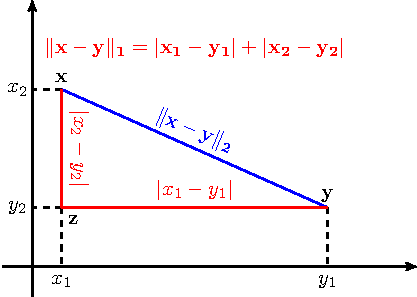
\includegraphics[width = .5\textwidth]{norm12.pdf}
			\caption{Minh họa norm 1 và norm 2}
			\label{fig:norm12}
		\end{figure}
		Norm 2 (màu xanh) chính là đường thằng "chim bay" nối giữa hai vector $\mathbf{x} $ và $\mathbf{y}$. Khoảng cách norm 1 giữa hai điểm này (màu đỏ) có thể diễn giải như là đường đi từ $\mathbf{x} $ tới $\mathbf{y}$ trong một thành phố mà đường phố tạo thành hình bàn cờ. Chúng ta chỉ có cách đi dọc theo cạnh của bàn cờ mà không được đi thẳng. 
 	
 	\item Khi $p \rightarrow \infty $, ta có norm $p$ chính là trị tuyệt đối của phần tử lớn nhất của vector đó:
		\begin{equation} 
		\|\mathbf{x}\|_{\infty} = \max_{i = 1, 2, \dots, n} \|x_i\|
		\end{equation} 
 
\end{enumerate} 
 
\subsection{Chuẩn của ma trận}
Với một ma trận $\mathbf{A} \in \mathbb{R}^{m\times n}$, chuẩn thường được dùng nhất là chuẩn Frobenius, ký hiệu là $\|\mathbf{A}\|_F$ là căn bậc hai của tổng bình phương tất cả các phần tử của ma trận đó.  
\begin{equation*} 
\|\mathbf{A}\|_F = \sqrt{\sum_{i = 1}^m \sum_{j = 1}^n a_{ij}^2} 
\end{equation*} 
 
 
 
 
\section{Đạo hàm của hàm nhiều biến }
Trong mục này, chúng ta sẽ giả sử rằng các đạo hàm tồn tại. Chúng ta sẽ xét hai trường hợp: i) Hàm số nhận giá trị là ma trận (vector) và cho giá trị là một số thực vô hướng; và ii) Hàm số nhận giá trị là một số vô hướng hoặc vector và cho giá trị là một vector.  
 
 
\subsection{Hàm cho giá trị là một số vô hướng}
 
Đạo hàm (gradient) của một hàm số $f(\mathbf{x}): \mathbb{R}^n \rightarrow \mathbb{R}$ \textbf{theo vector} $\mathbf{x}$ được định nghĩa như sau:  
 
\begin{equation} 
	\label{eqn:grvector1}
	\nabla_{\mathbf{x}} f(\mathbf{x}) \triangleq  
	\left[ 
	\begin{matrix} 
	\frac{\partial f(\mathbf{x})}{\partial x_1} \\\ 
	\frac{\partial f(\mathbf{x})}{\partial x_2} \\\ 
	\vdots \\\ 
	\frac{\partial f(\mathbf{x})}{\partial x_n} 
	\end{matrix} 
	\right] \in \mathbb{R}^n 
\end{equation} 
trong đó $\frac{\partial f(\mathbf{x})}{\partial x_i}$ là đạo hàm của hàm số theo thành phần thứ $i$ của vector $\mathbf{x}$. Đạo hàm này được lấy khi giả sử tất cả các biến còn lại là hằng số. 
 
Nếu không có thêm biến nào trong hàm số, $\nabla_{\mathbf{x}}f(\mathbf{x})$ thường được viết gọn là $\nabla f(\mathbf{x})$. 
 
Điều quan trọng cần nhớ: \textbf{đạo hàm của hàm số này là một vector có cùng chiều với vector đang lấy đạo hàm}. Tức nếu vector viết ở dạng cột thì đạo hàm cũng phải viết ở dạng cột.  
 
Đạo hàm bậc hai (second-order gradient) của hàm số trên còn được gọi là \textit{Hessian} và được định nghĩa như sau:  
 
\begin{equation} 
\label{eqn:hessian1}
\nabla^2 f(\mathbf{x}) \triangleq 
\left[ 
\begin{matrix} 
    \frac{\partial^2 f(\mathbf{x})}{\partial x_1^2} & \frac{\partial^2 f(\mathbf{x})}{\partial x_1x_2} & \dots & \frac{\partial^2 f(\mathbf{x})}{\partial x_1x_n} \\\  
    \frac{\partial^2 f(\mathbf{x})}{\partial x_2x_1} & \frac{\partial^2 f(\mathbf{x})}{\partial x_2^2} & \dots & \frac{\partial^2 f(\mathbf{x})}{\partial x_2x_n} \\\  
    \vdots & \vdots & \ddots & \vdots \\\ 
    \frac{\partial^2 f(\mathbf{x})}{\partial x_nx_1} & \frac{\partial^2 f(\mathbf{x})}{\partial x_nx_2} & \dots & \frac{\partial^2 f(\mathbf{x})}{\partial x_n^2} \\\  
\end{matrix} 
\right] \in \mathbb{S}^{n}
\end{equation}  
với $\mathbb{S}^{n} \in \mathbb{R}^{n \times n}$ là tập các ma trận vuông đối xứng có số cột là $n$. 

Đạo hàm của một hàm số $f(\mathbf{X}): \mathbb{R}^{n \times m} \rightarrow \mathbb{R}$ \textbf{theo ma trận} $\mathbf{X}$ được định nghĩa là:  
\begin{equation}
\label{eqn:grmatrix1} 
\nabla f(\mathbf{X}) = 
\left[ 
\begin{matrix} 
    \frac{\partial f(\mathbf{X})}{\partial x_{11}} & \frac{\partial f(\mathbf{X})}{\partial x_{12}} & \dots & \frac{\partial f(\mathbf{X})}{\partial x_{1m}} \\\ 
    \frac{\partial f(\mathbf{X})}{\partial x_{21}} & \frac{\partial f(\mathbf{X})}{\partial x_{22}} & \dots & \frac{\partial f(\mathbf{X})}{\partial x_{2m}} \\\ 
    \vdots & \vdots & \ddots & \vdots \\\ 
    \frac{\partial f(\mathbf{X})}{\partial x_{n1}} & \frac{\partial f(\mathbf{X})}{\partial x_{n2}} & \dots & \frac{\partial f(\mathbf{X})}{\partial x_{nm}}  
\end{matrix} 
\right] \in \mathbb{R}^{n \times m}
\end{equation} 
 
Một lần nữa, đạo hàm của một hàm số theo ma trận là một ma trận có chiều giống với ma trận đó. 
 
Hiểu một cách đơn giản, đạo hàm của một hàm số (có đầu ra là 1 số vô hướng) theo một ma trận được tính như sau. Trước tiên, tính đạo hàm của hàm số đó theo từng thành phần của ma trận \textit{khi toàn bộ các thành phần khác được giả sử là hằng số}. Tiếp theo, ta \textit{ghép} các đạo hàm thành phần tính được thành một ma trận đúng theo thứ tự như trong ma trận đó. Chú ý rằng vector là một trường hợp của ma trận.  
 
\textbf{Ví dụ:} Xét hàm số: $f: \mathbb{R}^2 \rightarrow \mathbb{R}$, $f(\mathbf{x}) = x_1 ^2 + 2x_1x_2 + \sin(x_1) + 2$.  
 
Đạo hàm bậc nhất theo $\mathbf{x}$ của hàm số đó là:  
\begin{equation*} 
\nabla f(\mathbf{x}) = 
\left[ 
\begin{matrix} 
    \frac{\partial f(\mathbf{x})}{\partial x_1} \\\ 
    \frac{\partial f(\mathbf{x})}{\partial x_2} 
\end{matrix} 
\right] = \left[ 
\begin{matrix} 
    2x_1 + 2x_2 + \cos(x_1) \\\ 
    2x_1 
\end{matrix} 
\right] 
\end{equation*} 
 
Đạo hàm bậc hai theo $\mathbf{x}$, hay \textit{Hessian} là:  
\begin{equation*} 
\nabla^2 f(\mathbf{x}) =  
\left[ 
\begin{matrix} 
    \frac{\partial^2 f(\mathbf{x})}{\partial x_1^2} & \frac{\partial f^2(\mathbf{x})}{\partial x_1x_2} \\\ 
    \frac{\partial^2 f(\mathbf{x})}{\partial x_2x_1} & \frac{\partial f^2(\mathbf{x})}{\partial x_2^2} 
\end{matrix} 
\right] = 
\left[ 
\begin{matrix} 
    2 - \sin(x_1) & 2 \\\ 
    2 & 0  
\end{matrix} 
\right] 
\end{equation*} 
Chú ý rằng \textit{Hessian} luôn là một ma trận đối xứng.  
 
 
 
\subsection{Hàm cho giá trị là một vector }
 
Những hàm số cho giá trị là một vector được gọi là \textit{vector-valued function} trong tiếng Anh.  
 
Giả sử một hàm số với \textbf{đầu vào là một số thực} $v(x): \mathbb{R} \rightarrow \mathbb{R}^n $: 
\begin{equation} 
\label{eqn:vectorvalued}
v(x) =  
\left[ 
\begin{matrix} 
    v_1(x) \\\ 
    v_2(x) \\\ 
    \vdots \\\ 
    v_n(x) 
\end{matrix} 
\right] 
\end{equation} 
Đạo hàm của nó là một \textbf{vector hàng} như sau:  

\begin{equation} 
\label{eqn:grvectorvalued}
\nabla v(x) \triangleq  
\left[ 
\begin{matrix} 
    \frac{\partial v_1(x)}{\partial x} & \frac{\partial v_2(x)}{\partial x} & \dots & \frac{\partial v_n(x)}{\partial x} 
\end{matrix} 
\right]
\end{equation} 
Đạo hàm bậc hai của hàm số này có dạng: 
 
\begin{equation} 
	\label{eqn:hessianvectorvalued}
	\nabla^2 v(x) \triangleq  
	\left[ 
	\begin{matrix} 
	    \frac{\partial^2 v_1(x)}{\partial x^2} & \frac{\partial^2 v_2(x)}{\partial x^2} & \dots & \frac{\partial^2 v_n(x)}{\partial x^2} 
	\end{matrix} 
	\right] 
\end{equation} 
 
\textbf{Ví dụ:} Cho vector $\mathbf{a} \in \mathbb{R}^n$ và \textit{vector-valued function} $v(x) = x\mathbf{a}$, thế thì: 
\begin{equation} 
\nabla v(x) = \mathbf{a}^T, ~~~ \nabla^2 v(x) = \mathbf{0} \in \mathbb{R}^{n\times n} 
\end{equation} 
với $\mathbf{0}$ là ma trận với các thành phần đều là 0.  

Xét một \textit{vector-valued function} với \textbf{đầu vào là một vector} $h(\mathbf{x}):\mathbb{R}^k \rightarrow \mathbb{R}^n$, đạo hàm bậc nhất của nó là: 
\begin{eqnarray} 
\label{eqn:gdvectorvector}
\nabla h(\mathbf{x}) &\triangleq & 
\left[ 
\begin{matrix} 
    \frac{\partial h_1(\mathbf{x})}{\partial x_1} & \frac{\partial h_2(\mathbf{x})}{\partial x_1} & \dots & \frac{\partial h_n(\mathbf{x})}{\partial x_1} \\\  
    \frac{\partial h_1(\mathbf{x})}{\partial x_2} & \frac{\partial h_2(\mathbf{x})}{\partial x_2} & \dots & \frac{\partial h_n(\mathbf{x})}{\partial x_2} \\\  
    \vdots & \vdots & \ddots & \vdots \\\ 
    \frac{\partial h_1(\mathbf{x})}{\partial x_k} & \frac{\partial h_2(\mathbf{x})}{\partial x_k} & \dots & \frac{\partial h_n(\mathbf{x})}{\partial x_k} 
\end{matrix} 
\right]\\
\label{eqn:gdvectorvector_short}
& = &  
\left[ 
\begin{matrix} 
    \nabla h_1(\mathbf{x}) & \nabla h_2(\mathbf{x}) & \dots & \nabla h_n(\mathbf{x}) 
\end{matrix} 
\right] \in \mathbf{R}^{k\times n} 
\end{eqnarray} 
 
 
\textbf{Một quy tắc dễ nhớ ở đây là nếu một hàm số} $g: \mathbb{R}^m \rightarrow \mathbb{R}^n$ \textbf{thì đạo hàm của nó là một ma trận thuộc} $\mathbb{R}^{m \times n}$. 
 
Đạo hàm bậc hai của hàm số trên là một \textit{ma trận ba chiều}, tôi xin không đề cập ở đây.  
 

<hr> 
Với các hàm số \textit{matrix-valued} nhận giá trị đầu vào là ma trận, tôi cũng xin không đề cập ở đây. Tuy nhiên, ở phần dưới, khi tính toán đạo hàm cho các hàm cho giá trị là số thực, chúng ta vẫn có thể sẽ sử dụng khái niệm này. 
 
Trước khi đến phần tính đạo hàm của các hàm số thường gặp, chúng ta cần biết hai tính chất quan trọng khá giống với đạo hàm của hàm một biến được học trong chương trình cấp ba.  
 
 
\subsection{Hai tính chất quan trọng }
 
 
\subsubsection{Product rules}
Để cho tổng quát, ta giả sử biến đầu vào là một ma trận (vector và số thực là các trường hợp đặt biệt của ma trận). Giả sử rằng các hàm số có chiều phù hợp để các phép nhân thực hiện được. Ta có:  
 
\begin{equation} 
\label{eqn:productrules}
\nabla\left( f(\mathbf{X})^Tg(\mathbf{X}) \right) = \left(\nabla f(\mathbf{X})\right) g(\mathbf{X}) + \left(\nabla g(\mathbf{X})\right) f(\mathbf{X})  
\end{equation} 
 
Biểu thức này giống như biểu thức chúng ta đã quá quen thuộc: 
\begin{equation*} 
\left(f(x)g(x)\right)' = f'(x)g(x) + g'(x)f(x) 
\end{equation*} 
Chú ý rằng với vector và ma trận, chúng ta không được sử dụng tính chất giao hoán.  
 
 
\subsubsection{Chain rules }
Khi có các hàm hợp thì: 
\begin{equation} 
\label{eqn:chainrules}
\nabla_{\mathbf{X}} g(f(\mathbf{X})) = \nabla_{\mathbf{X}} f^T \nabla_{f}g  
\end{equation} 
 
Quy tắc này cũng giống với quy tắc trong hàm một biến:  
\begin{equation*} 
(g(f(x))' = f'(x)g'(f) 
\end{equation*} 
Nhắc lại rằng khi tính toán với ma trận, chúng ta cần chú ý tới chiều của các ma trận, và nhân ma trận không có tính chất giao hoán.  
 
\subsection{Đạo hàm của các hàm số thường gặp }
 
\subsubsection{$f(\mathbf{x}) = \mathbf{a}^T\mathbf{x}$}
 
Giả sử $\mathbf{a}, \mathbf{x} \in \mathbb{R}^n$, ta viết lại: 
\begin{equation*} 
f(\mathbf{x}) = \mathbf{a}^T\mathbf{x} = a_1 x_1 + a_2 x_2 + \dots + a_nx_n 
\end{equation*} 
Có thể nhận thấy rằng: 
\begin{equation*} 
\frac{\partial f(\mathbf{x})}{\partial x_i} = a_i, ~ \forall i = 1, 2\dots, n 
\end{equation*} 
Vậy nên: 
\begin{equation*} 
\nabla f(\mathbf{x}) =  
\left[ 
\begin{matrix} 
    a_1 \\\ 
    a_2 \\\ 
    \vdots \\\ 
    a_n 
\end{matrix} 
\right] = \mathbf{a}
\end{equation*} 
 
Thêm nữa, vì $\mathbf{a}^T\mathbf{x} = \mathbf{x}^T\mathbf{a}$ nên: 
\begin{equation*} 
\nabla (\mathbf{x}^T\mathbf{a}) = \mathbf{a} 
\end{equation*} 
 
 
\subsubsection{$f(\mathbf{x}) = \mathbf{Ax}$}
Đây là một \textit{vector-valued function} $f: \mathbb{R}^n \rightarrow \mathbb{R}^{m} $ với $\mathbf{x} \in \mathbb{R}^n, \mathbf{A} \in \mathbb{R}^{m\times n}$. Giả sử rằng $\mathbf{a}_i$ là \textbf{hàng} thứ $i$ của ma trận $\mathbf{A}$. Ta có:  
\begin{equation*} 
\mathbf{Ax}  =  
\left[ 
\begin{matrix} 
    \mathbf{a}_1\mathbf{x} \\\ 
    \mathbf{a}_2\mathbf{x} \\\ 
    \vdots\\\ 
    \mathbf{a}_m\mathbf{x}  
\end{matrix} 
\right] 
\end{equation*} 
Theo định nghĩa $(13.2)$, và công thức $(17)$, ta có thể suy ra: 
\begin{equation} 
\label{eqn:gdAx}
\nabla_{\mathbf{x}} (\mathbf{Ax}) =  
\left[ 
\begin{matrix} 
    \mathbf{a}_1^T & \mathbf{a}_2^T & \dots & \mathbf{a}_m^T 
\end{matrix} 
\right] = \mathbf{A}^T 
\end{equation} 
 
Từ đây ta có thể suy ra đạo hàm của hàm số $f(\mathbf{x}) = \mathbf{x} = \mathbf{Ix}$, với $\mathbf{I}$ là ma trận đơn vị với chiều phù hợp, là: 
\begin{equation*} 
\nabla \mathbf{x} = \mathbf{I} 
\end{equation*} 
 
\subsubsection{$f(\mathbf{x}) = \mathbf{x}^T\mathbf{A} \mathbf{x}$}
với $\mathbf{x} \in \mathbb{R}^n, \mathbf{A} \in \mathbb{R}^{n\times n}$. Áp dụng Product rules $(14)$ ta có: 
\begin{eqnarray} 
	\nonumber
	\nabla f(\mathbf{x}) &=& \nabla \left(\left(\mathbf{x}^T\right) \left(\mathbf{Ax}\right)\right) \\\ 
				\nonumber
                     &=& \left(\nabla (\mathbf{x})\right) \mathbf{Ax} + \left(\nabla (\mathbf{Ax})\right)\mathbf{x} \\\  
					\nonumber
                     & = & \mathbf{IAx} + \mathbf{A}^T\mathbf{x} \\\ 
                     \label{eqn:gdxTAx}
                     & = & (\mathbf{A} + \mathbf{A}^T)\mathbf{x} 
\end{eqnarray} 
 
 
Từ \eqref{eqn:gdxTAx} và \eqref{eqn:gdAx}, ta có thể suy ra:  
\begin{math} 
\nabla^2 \mathbf{x}^T\mathbf{Ax} = \mathbf{A}^T + \mathbf{A} 
\end{math} 
 
Nếu $\mathbf{A}$ là một ma trận đối xứng, ta sẽ có: 
\begin{equation} 
\nabla \mathbf{x}^T\mathbf{A}\mathbf{x} = 2\mathbf{Ax}, ~~~
\nabla^2 \mathbf{x}^T\mathbf{Ax} = 2\mathbf{A} 
\end{equation} 
 
Nếu $\mathbf{A}$ là ma trận đơn vị, tức $f(\mathbf{x}) = \mathbf{x}^T\mathbf{Ix} = \mathbf{x}^T\mathbf{x} = \|\mathbf{x}\|_2^2$, ta có: 
\begin{equation} 
\nabla \|\mathbf{x}\|_2^2 = 2\mathbf{x},~~~
\nabla^2 \|\mathbf{x}\|_2^2 = 2\mathbf{I} 
\end{equation} 
 
 
\subsubsection{$f(\mathbf{x}) = \|\mathbf{Ax} - \mathbf{b}\|_2^2 $}
Có hai cách tính đạo hàm của hàm số này: 
 
\textbf{Cách 1:} 
Trước hết, biến đổi: 
\begin{eqnarray} 
	\nonumber
	f(\mathbf{x}) &=& \|\mathbf{Ax} - \mathbf{b}\|_2^2 = (\mathbf{Ax} - \mathbf{b})^T(\mathbf{Ax} - \mathbf{b}) = (\mathbf{x}^T\mathbf{A}^T - \mathbf{b}^T) (\mathbf{Ax} - \mathbf{b}) \\\ \nonumber
	&=& \mathbf{x}^T\mathbf{A}^T\mathbf{Ax} - 2 \mathbf{b}^T\mathbf{Ax} + \mathbf{b}^T\mathbf{b} 
\end{eqnarray} 
Lấy đạo hàm cho từng số hạng rồi cộng lại ta có:  
\begin{equation*} 
\nabla \|\mathbf{Ax} - \mathbf{b}\|_2^2 = 2\mathbf{A}^T\mathbf{A}\mathbf{x} - 2\mathbf{A}^T\mathbf{b} = 2\mathbf{A}^T(\mathbf{Ax} - \mathbf{b}) 
\end{equation*} 
 
\textbf{Cách 2:} Dùng Chain rule. 
Sử dụng $\nabla (\mathbf{Ax} - \mathbf{b}) = \mathbf{A}^T$ và $\nabla \|\mathbf{x}\|_2^2 = 2\mathbf{x}$ và công thức chain rules \eqref{eqn:chainrules}, ta sẽ thu được kết quả tương tự.  
 
 
\subsubsection{$f(\mathbf{x}) = \mathbf{a}^T\mathbf{x}\mathbf{x}^T\mathbf{b}$}
Bằng cách viết lại $f(\mathbf{x}) = (\mathbf{a}^T\mathbf{x})(\mathbf{x}^T\mathbf{b})$, ta có thể dùng Product rules $(14)$ và ra kết quả:  
\begin{equation*} 
	\nabla (\mathbf{a}^T\mathbf{x}\mathbf{x}^T\mathbf{b}) = \mathbf{a} \mathbf{x}^T\mathbf{b} +  \mathbf{b}\mathbf{a}^T\mathbf{x} = \mathbf{ab}^T\mathbf{x} + \mathbf{b}\mathbf{a}^T\mathbf{x}= (\mathbf{ab}^T + \mathbf{ba}^T)\mathbf{x} 
\end{equation*} 
trong đây tôi đã sử dụng tính chất $\mathbf{y}^T\mathbf{z} = \mathbf{z}^T\mathbf{y}$ và tích của một số thực với một vector cũng bằng tích của vector và số thực đó.  
 
 
\subsection{Bảng các đạo hàm thường gặp}
 
\subsubsection{Cho vector }
 
\begin{table}[h!]
\centering
\caption{Đạo hàm theo vector}
\label{my-label}
\begin{tabular}{|c|c|}
\hline
$f(\mathbf{x}) $                                                                          & $ \nabla f(\mathbf{x}) $                                         \\ \hline
$\mathbf{a}^T \mathbf{x} $                                                                & $\mathbf{a}$                                                     \\ \hline
$\mathbf{x}^T\mathbf{Ax}$                                                                 & $\mathbf{A} + \mathbf{A}^T) \mathbf{x}$                          \\ \hline
$\mathbf{x}^T \mathbf{x} = \|\mathbf{x}\|_2^2 $ & $2\mathbf{x}$                                                   \\ \hline
$ \|\mathbf{Ax-b} \|_2^2 $                                                                & $ 2\mathbf{A}^T (\mathbf{Ax - b})$                               \\ \hline
$\mathbf{a}^T\mathbf{x}^T\mathbf{xb} $                                                    & $2\mathbf{a}^T\mathbf{bx} $                                      \\ \hline
$\mathbf{a}^T\mathbf{x}\mathbf{x}^T\mathbf{b} $                                           & $ (\mathbf{a}\mathbf{b}^T + \mathbf{b}\mathbf{a}^T) \mathbf{x} $ \\ \hline
\end{tabular}
\end{table}


 
\subsubsection{Cho ma trận}
 

 \begin{table}[h!]
\centering
\caption{Đạo hàm theo ma trận}
\label{my-label}
\begin{tabular}{|c|c|}
\hline
$f(\mathbf{X}) $                                   & $ \nabla f(\mathbf{X}) $                      \\ \hline
$ \|\mathbf{X}\|_F^2$ & $2\mathbf{X}$ \\\hline
$ \mathbf{AX}$ & $\mathbf{A}^T$ \\\hline
$ \|\mathbf{AX - B}\|_F^2$ & $2\mathbf{A}^T(\mathbf{AX - B})$ \\\hline
$ \|\mathbf{XA - B}\|_F^2$ & $2(\mathbf{XA-B})\mathbf{A}^T$ \\\hline
$ \mathbf{a}^T \mathbf{X}^T \mathbf{Xb}$           & $ \mathbf{X}(\mathbf{ab}^T + \mathbf{ba}^T)$ \\ \hline
$ \mathbf{a}^T \mathbf{X} \mathbf{X}^T \mathbf{b}$ & $ (\mathbf{ab}^T + \mathbf{ba}^T)\mathbf{X},$ \\ \hline
$ \mathbf{a}^T \mathbf{Y} \mathbf{X}^T \mathbf{b}$ & $ \mathbf{b}\mathbf{a}^T \mathbf{Y}$         \\ \hline
$ \mathbf{a}^T \mathbf{Y}^T \mathbf{X} \mathbf{b}$ & $ \mathbf{Y}\mathbf{a}\mathbf{b}^T$          \\ \hline
$ \mathbf{a}^T \mathbf{X} \mathbf{Y}^T \mathbf{b}$ & $ \mathbf{a}\mathbf{b}^T\mathbf{Y}$          \\ \hline
$ \mathbf{a}^T \mathbf{X}^T \mathbf{Y} \mathbf{b}$ & $ \mathbf{Y}\mathbf{b}\mathbf{a}^T$          \\ \hline
\end{tabular}
\end{table}


\subsection{Tài liệu tham khảo }
[1] \href{https://ccrma.stanford.edu/~dattorro/matrixcalc.pdf}{Matrix calculus} 
 
 
 

\end{document}